\chapter{描述}\label{description}

由前两章内容可知,实体链接的一般流程包括指称识别、候选实体生成和实体消岐。
其中实体消岐的部分最有挑战也最为关键。
整个实体消岐的过程在有些文献\cite{shen2015entity}中也称为``候选实体排名'',对字符串指称的候选实体进行排名,最终排名最高的实体被选为指称的对应参考实体。
这个排名的过程与网页排名算法 PageRank\cite{page1999pagerank} 类似。
由表格的特点可知,单元格之间往往存在一定的语义相关性,这种语义相关性让两个单元格中的字符串指称关联在一起。
在知识库中,不同的实体之间也可能存在一定的语义相关性,同样,指称和实体之间也是可能语义相关的。
相互关联的字符串指称的链接结果可能会互相影响,为了充分利用这些语义相关性,马尔科夫链模型\cite{stewart1994introduction}是一个好选择。
马尔科夫链可以用来捕捉指称与实体、实体与实体之间的语义相关性,从而提高实体链接的质量。
在我的两个方法中,实体消岐的算法都运用了马尔科夫链模型和一个个性化的 PageRank 算法\cite{haveliwala2003topic}\cite{langville2011google},而 PageRank 算法建立在随机游走模型上\cite{haveliwala2003topic},并且随机游走就是一种马尔科夫链的例子,所以我的方法其实就是在马尔科夫链模型上进行随机游走。
马尔科夫链可以用图表示,因此毕设中的两个方法也可以称为是基于图的随机游走算法。
在本章中,我会先介绍马尔科夫链模型和随机游走模型,然后详细地描述两个方法的细节。


\section{马尔可夫链}
马尔可夫链,为状态空间中经过从一个状态到另一个状态的转换的随机过程。
该过程要求具备``无记忆''的性质:下一状态的概率分布只能由当前状态决定,在时间序列中它前面的事件均与之无关。
这种``无记忆性''称为马尔可夫性质。
图~\ref{markov_chain} 中即为一个马尔科夫链的例子。
在马尔可夫链的每一步,根据概率分布,可以从一个状态变到另一个状态,也可以保持当前状态。
状态的改变叫做转移,与不同的状态改变相关的概率叫做转移概率。
随机漫步就是马尔可夫链的例子。
随机漫步中每一步的状态是在图形中的点,每一步可以移动到任何一个相邻的点,在这里移动到每一个点的概率都是相同的 (无论之前漫步路径是如何的)。\par

% Fig 
\begin{figure}[htbp]
\centering
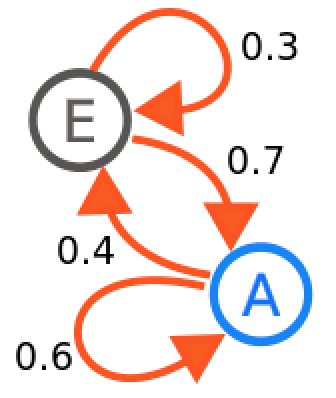
\includegraphics[width=0.15\textwidth]{img/markov_chain}
\caption{一个具有两个转换状态的马尔可夫链}
\label{markov_chain}
\end{figure}

若状态空间是有限的,则马尔科夫链的转移概率分布可以矩阵表示,该矩阵称为转移矩阵,记为 $\bm{P}$,在后文中迭代概率繁殖中也称为概率转移矩阵。
如果 $\bm{P}$ 是一步转移矩阵,$\bm{P}^k$ 就是 $k$ 步转移后的转移矩阵。
由马尔科夫链\footnote{\url{https://en.wikipedia.org/wiki/Markov_chain}}在有限状态空间内的性质\cite{tauchen1986finite}可知,如果转移矩阵 $\bm{P}$ 不可约且非周期,则 $\bm{P}$ 会收敛到一个独立的稳态分布 $\bm{\pi}$。
用公式表示如下:
\begin{equation}
	\lim_{k \rightarrow \infty} \bm{P}^k = \bm{1} \bm{\pi}
\label{pk}
\end{equation}
其中 $\bm{1}$ 是一个列向量每个元素都为1。
还有一个关于马尔科夫链的重要性质是一个正转移矩阵 (矩阵中每个元素都为正) 是不可约和非周期的。
这些性质都是~\ref{single} 节中迭代概率传播算法的理论基础。
它们保证了在实体消岐图上运行随机游走算法能够在有限次迭代内达到收敛。


\section{随机游走}
随机游走,是一种数学统计模型,由一连串的轨迹所组成,其中每一次都是随机的。
它能用来表示不规则的变动形式,如同一个人酒后乱步,所形成的随机过程记录。
通常,可以假设随机游走是以马尔可夫链或马可夫过程的形式出现。
在图~\ref{random_walk} 中是一个一维随机游走的例子。
PageRank\cite{page1999pagerank} 算法可以用随机游走模型来解释\cite{haveliwala2003topic}。
PageRank 通过 Web 上的超链接关系来确定一个页面的等级,用于计算网页的相关性和重要性。

% Fig 
\begin{figure}[htbp]
\centering
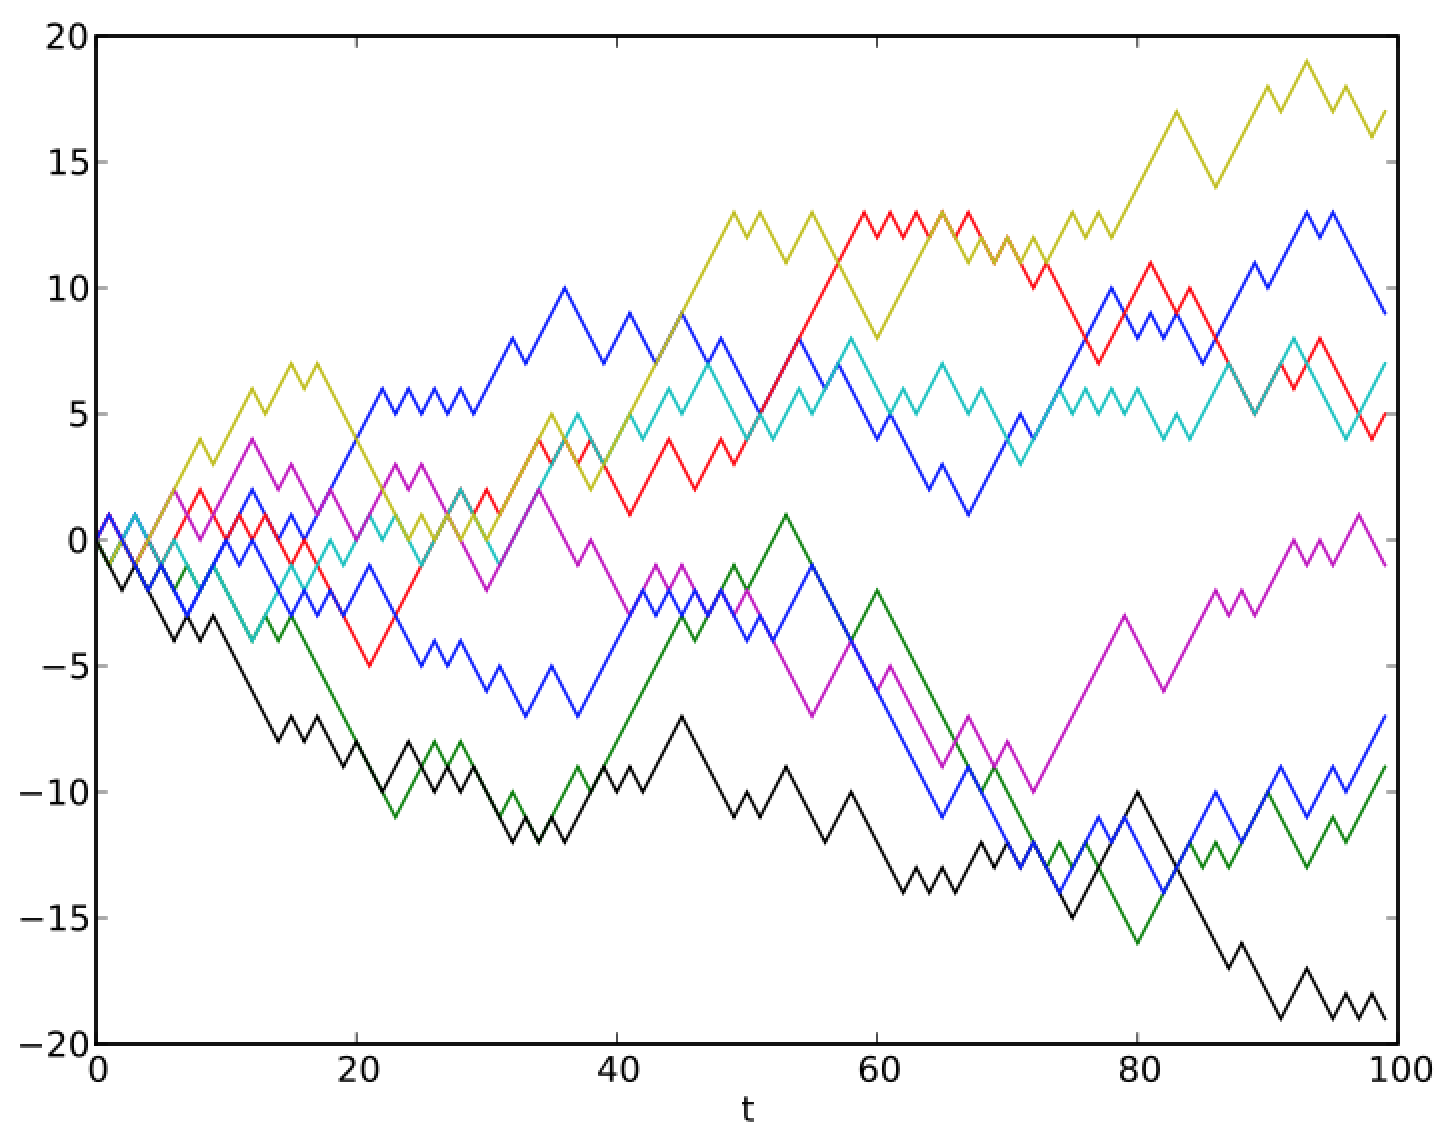
\includegraphics[width=0.35\textwidth]{img/random_walk}
\caption{一维的随机游走。纵轴表示当前的位置,横轴表示时间步数。}
\label{random_walk}
\end{figure}


\section{方法一: 两步走}\label{approach1}

方法一包含两个主要的步骤:首先使用各个单知识库进行实体链接,然后运行多知识库间的 ``sameAs'' 关系来优化单知识库的链接结果。

% Fig 
\begin{figure}[htbp]
\centering
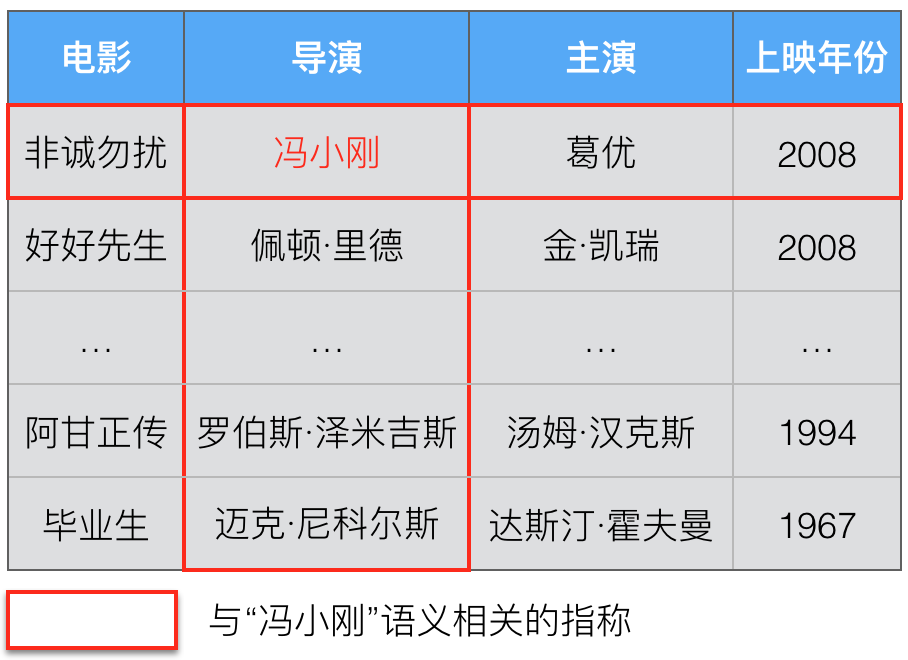
\includegraphics[width=0.6\textwidth]{img/table}
\caption{一个表格同行同列中的指称具有语义相关性的示例}
\label{table}
\end{figure}

\subsection{单知识库表格实体链接}\label{single}

\noindent\textbf{指称识别} \ 
任何实体链接系统的第一步是识别出潜在的字符串指称,它们能够被链接到知识库中的参考实体。
给定来自输入的表格中每个单元格的文本内容,$t_q$,系统将 $t_q$ 中满足一定条件的最长的短语 $s$ 识别为潜在的指称。
这个条件就是对于某些实体 $e$,字符串 $s$ 能链接到该实体的概率 $P(e|s)$ 非零。
如果 $s$ 的长度小于 $t_q$ 的长度,系统会在 $s$ 之后发现长度最长的短语,并以此类推。
例如,对于一个单元格的文本 ``习近平 \& 彭丽媛'',系统会识别出到两个潜在的指称:一个是``习近平'',另一个是``彭丽媛''。\newline


\noindent\textbf{候选实体生成} \ 
对于表格单元格中的每个字符串指称,首先需要从给定的海量的知识库实体中找出一些可能成为该指称参考实体的实体,来缩小实体链接的范围。
这样的实体称为字符串指称的候选实体。这样的过程叫做生成候选实体。
我讲每个指称分割到单词级别,所以每个指称能被表示为一个单词集合。
如果给定知识库中的一个实体 $e$ 或者 $s$ 在 BabelNet\cite{navigli2010babelnet} (一个全网域多语种同义词辞典) 中的一个同义词包含某个指称 $m$ 的分割单词集合中的至少一个单词,那么实体 $e$ 就被认为是指称 $m$ 的一个候选参考实体。
举个例子,字符串指称``苹果''有这样的一些候选实体:``苹果'',``苹果派'',``苹果 [水果]'',``苹果 [智能手机品牌]''。
候选实体生成的结果就是每个指称都可能指向一个候选实体集合。
在实际操作过程中,除了指称与实体的包含关系,我还考虑了二者之间的字符串相似度 (计算公式在后面会提到),设置了一个字符串相似度的阈值。
一般来说,与指称的字符串相似度很低的实体,很有可能表示的是跟指称完全不同的事物,即便它们有包含关系。
所以如果实体 $e$ 和指称 $m$ 的字符串相似度低于阈值,即使 $e$ 包含 $m$,也不将该实体 $e$ 添加进 $m$ 的候选实体集合。
比如,对于指称``苹果'',在知识库中有这样的一个实体``苹果红蜘蛛'',显然二者不可能相链接,虽然这个实体里包含了``苹果''二字,但是由于二者的字符串相似度太低,这样的实体就被剔除了。
\newline

\noindent\textbf{实体消岐} \ 
一个指称的候选实体集合可能是空集,也可能包含一个或多个候选实体。
当候选实体集合是空集的时候,那么这个指称是不可链接的,给它打上``NIL''标签。
当候选实体集合中包含多个候选实体的时候,哪个候选实体最有可能成为字符串指称的对应参考实体就成了需要考虑的问题。
从指称的候选实体集合中挑选一个最合适的实体作为指称在给定知识库中的对应参考实体就是实体消岐的目标。
就像图~\ref{table} 中所示,可以发现在同一行或者同一列的指称很可能是语义相关的。
换句话中,出现在同一个 Web 表格中的任意两个指称之间可能存在着一些潜在的联系。
因此,我选择使用一个基于图的随机游走算法来对一个表格中的所有指称进行联合消岐。
实体消岐分为三个子步骤:
\begin{enumerate}[a)]
\item 首先,对于每张给定的表格,建立一个实体消岐图 (Entity Disambiguation Graph),这张图只使用表格中的指称和它们的候选实体作为图中的结点。构建实体消岐图的过程即为将表格中的指称和其候选实体建模成马尔科夫链的过程。
\item 然后,在每个构筑好的实体消岐图上,计算每个指称的初始权重值用于联合消岐,同时将不同结点间的语义相关度计算出来作为实体链接影响因子 (EL Impact Factors) 来决定到底哪个实体是给定的指称的对应参考实体。
\item 最后,计算实体消岐图的概率转移矩阵并运行随机游走算法,具体来说,就是使用实体链接影响因子进行迭代概率传播 (Iterative Probability Propagation),直到实体结点上的概率收敛,这里的迭代概率传播中的``概率''指的是每个实体结点上的概率,它代表该实体成为给定指称的对应参考实体的概率,最后基于这些实体结点上的概率来得到最终的实体链接结果,指称结点的候选实体结点中概率最高的结点胜出成为指称的对应参考实体。
\end{enumerate}


\noindent\newline 在接下来的部分中,我会讲述这三个子步骤的来龙去脉。

a) \textbf{构建实体消岐图} \ 
对于每张给定的表格,建立一张实体消岐图 (Entity Disambiguation Graph),其包含两种类型的结点和两种类型的边,解释如下:
\begin{itemize}
  \item[$\bullet$] \textbf{指称结点}: 这些结点指的是 Web 表格中的字符串指称
  \item[$\bullet$] \textbf{实体结点}: 这些结点表示指称在给定知识库中的候选参考实体
  \item[$\bullet$] \textbf{指称-实体边}: 一条指称-实体边是一个指称和其候选参考实体集合中的一个实体之间的无向边
  \item[$\bullet$] \textbf{实体-实体边}: 一条实体-实体边是实体之间的无向边
\end{itemize}

一个构建好的实体消岐图的例子在图~\ref{edg} 中展示。
因为论文纸张空间所限,这里只画出了图~\ref{table} 中 Web 表格的实体消岐图的一部分,许多结点和边在图~ref{edg}中并没有显示。
每个指称和其候选实体集合中的每个实体间都有一条指称-实体边相连接。
比如指称``非诚勿扰''与它的2个候选实体``非诚勿扰 [电影]''、``非诚勿扰 [相亲节目]''之间都有指称-实体边相连接。
实体-实体边应该在图中所有实体结点间创建。
实体消岐图中的边是无向的,其实也可以理解为双向的,这在之后的迭代概率传播中概率转移矩阵的计算中会提到。
由实体消岐图的结构可知,一个指称结点如果是``NIL''的,那么它不与任何实体结点相连,换句话说,它没有任何相邻的结点。
在这里,两个结点通过一条边直接相连,那么我称这样的两个结点是``相邻''的。
一个指称结点的候选实体集合如果非空,那么它可能有一个或者多个相邻的实体结点。
而一个实体结点则与其所在的实体消岐图的所有其他实体结点相邻,与且仅与一个指称结点相邻,并且该实体结点是这个指称结点的候选实体之一。
需要额外说明的是,如果有两个指称结点的候选实体集合中有相同的知识库实体,在实体消岐图中建立的是两个不同的实体结点,即使它们代表的是同一个实体,而不是只建立一个实体结点。
构建实体消岐图的过程也就是将一张表格中的所有指称和其候选实体建模成一个马尔科夫链的过程。
\newline

% Fig 
\begin{figure}[htbp]
\centering
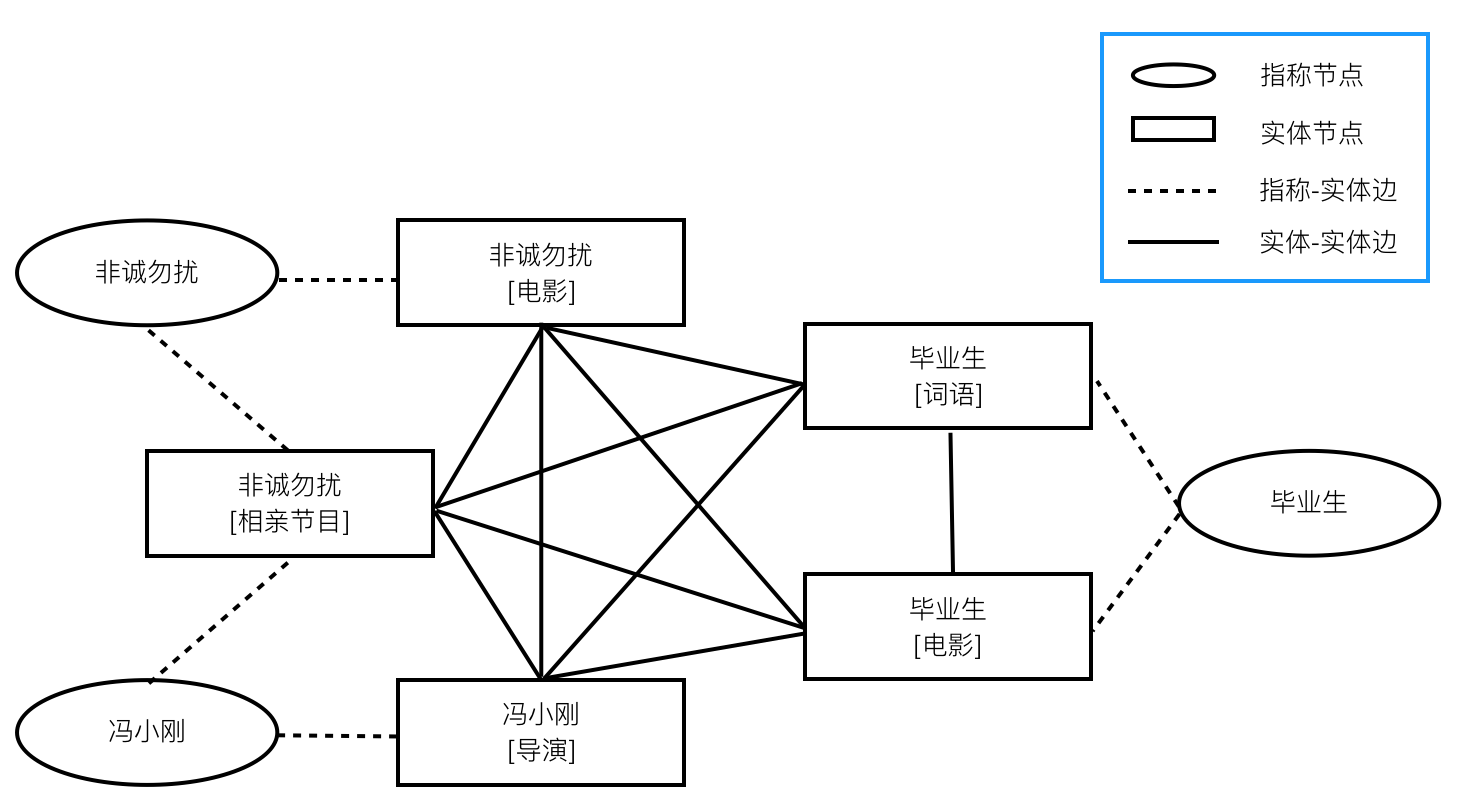
\includegraphics[width=0.9\textwidth]{img/edg}
\caption{一个构建好的实体消岐图示例}
\label{edg}
\end{figure}

b) \textbf{计算实体链接影响因子} \ 
在为给定的 Web 表格构建好实体消岐图之后,为每个结点和每条边上赋上一个概率值。
对于实体结点,结点上的概率表示它成为指称的对应参考实体的概率,在其被实体链接影响因子 (EL Impact Factors) 影响之前初始化为0。
实体链接影响因子实际上由2部分组成:
\begin{enumerate}[1)]
\item 指称结点的概率,它们代表了指称对于联合消岐的重要性
\item 边上的概率,即为结点间的语义相关度 (Semantic Relatedness)。
在本文中,认为每个指称都是地位平等的,所以当 Web 表格中有 k 个指称的时候,每个指称的重要性分值都初始化为 $\frac{1}{k}$。
因为在构建好的实体消岐图中有两种不同类型的边,指称-实体边与实体-实体边上的概率分别与指称-实体间的语义相关度和实体-实体间的语义相关度挂钩。
\end{enumerate}

对于\textbf{指称-实体间的语义相关度},我使用了两个特征来计算它,计算方式如下:
\begin{itemize}
	\item[$\bullet$] \textbf{字符串相似度特征} \ 
	假如一个指称 $m$ 和一个实体 $e$ 在字符串层面很相似,那么有可能 $e$ 是 $m$ 在给定知识库中的候选实体。
	因此,我把字符串相似度特征 $strSim(m,e)$ 定义为:
	\begin{equation}
	strSim(m,e)=1-\frac{Levenshtein(m,e)}{max\{|s|, |e|\}}
	\label{strsim}
	\end{equation}
	其中 $|m|$ 和 $|e|$ 分别是指称 $m$ 和实体 $e$ 的字符串长度。
	$Levenshtein(m,e)$ 代表 $|m|$ 和 $|e|$ 之间的莱文斯坦距离 (Levenshtein Distance\footnote{\url{https://en.wikipedia.org/wiki/Levenshtein_distance}}),是一个衡量两个字符串差异性的标准。
	如果指称 $m$ 和实体 $e$ 在字符串层面越相似,那么 $strSim(m,e)$ 的值会越高。
	\item[$\bullet$] \textbf{指称-实体的上下文相似度特征} \ 
	给定一个指称 $m$ 和其候选实体集合中的一个实体 $e$,假如两者是语义相关的,那么两者可能有相似的上下文 (Context)。
	在这里,为了获取给定指称 $m$ 的上下文,我先将 $m$ 所在的表格单元格的同行同列的其他单元格中的指称收集起来,然后再将这些收集到的指称分词,得到一个单词集合。
	我使用了当今顶级的中文分词工具``结巴中文分词\footnote{\url{https://github.com/fxsjy/jieba}}''来完成实验中的各种分词操作。
	最后,将这个单词集合中的所有单词作为 $m$ 的上下文并把它表示为 $menContext(m)$。
	对于实体 $e$ 的上下文,它来自知识库的两种类型的数据。
	一是知识库的信息盒属性 (Infobox Property)。
	打开任意一张知识库的实体页面,其中一般都会有一个包含实体的各种属性的表格,这就是信息盒。
	通过爬虫程序将知识库的所有的这种信息盒爬取下来,这就组成了信息盒属性数据,这些数据以 RDF\cite{munoz2014using} 三元组的格式存储,每个 RDF 三元组都由主语、谓语和宾语组成。
	我首先将所有包含实体 $e$ 的 RDF 三元组收集起来,如果 $e$ 在一个 RDF 三元组的主语中出现,那么将其宾语分词成一个单词集合。
	同理,如果 $e$ 在一个 RDF 三元组的宾语中出现,那么将其主语分词成一个单词集合。
	这样的单词集合是实体 $e$ 的上下文的一部分;
	二是知识库的摘要信息 (Abstract)。
	摘要信息一般位于知识库的实体页面的开头,是一个描述实体的段落。
	将知识库的所有的这种摘要信息爬取下来,就组成了摘要数据,这些数据同样是以 RDF 三元组的格式存储的,每个 RDF 三元组的主语是实体的名称,宾语是描述该实体的摘要。
	遍历知识库的整个摘要数据,将包含实体 $e$ 的 RDF 三元组收集起来,然后将这些三元组的宾语分词成一个单词集合。
	这样的单词集合构成了实体 $e$ 的上下文的另一部分。
	我用 $entContext(e)$ 来表示实体 $e$ 的上下文。
	为了计算指称 $m$ 和实体 $e$ 之间的指称-实体上下文相似度 $contSim_{me}(m,e)$,我应用了杰卡德相似度 (Jaccard Similaruty\footnote{\url{https://en.wikipedia.org/wiki/Jaccard_similarity}}),如下所示:
	\begin{equation}
	contSim_{me}(m,e)=\frac{|menContext(m)\bigcap{entContext(e)}|}{|menContext(m)\bigcup{entContext(e)}|}
	\end{equation}
\end{itemize}
对于给定的一个指称 $m$ 和一个实体 $e$,为了将二者之间的字符串相似度 $strSim(m,e)$ 和指称-实体上下文相似度 $contSim_{me}(m,e)$ 整合起来,我定义了如下公式所示的\textbf{指称-实体语义相关度} $SR_{me}(m,e)$:
\begin{equation}
SR_{me}(m,e)=c_1\times(\alpha_1 \cdot strSim(m,e) + \beta_1 \cdot contSim_{me}(m,e)) + c_2
\label{equation_srme}
\end{equation}
其中 $c_1$ 和 $c_2$ 是两个常量,在后面的迭代概率传播中的概率转移矩阵的计算中,需要保证实体消岐图的连通性,即边上的概率,或者说是结点间的语义相关度非零,所以为了保证指称 $m$ 和实体 $e$ 之间的语义相关度为非零,将 $c_1$ 和 $c_2$ 分别设为 0.99 和 0.01,这样 $SR_{me}(m,e)$ 至少为 0.01。
$\alpha_1$ 和 $\beta_1$ 分别是指称 $m$ 和实体 $e$ 之间的字符串相似度和指称-实体上下文相似度的权重值,在实验中,都设置为 0.5。
\newline

对于\textbf{实体-实体间的语义相关度},我也定义了如下两个特征来计算它:
\begin{itemize}
	\item[$\bullet$] \textbf{三元组关系特征} \ 
	本特征来自前面提到的知识库的信息盒属性数据,这些数据是以 RDF 三元组格式存储,每一条信息盒属性都是一个 RDF 三元组。
	如果两个实体处于同一个 RDF 三元组中,那么它们明显是语义相关的。
	因此,我用下面的公式来计算实体 $e_1$ 和实体 $e_2$ 之间的三元组关系特征 $IsRDF(e_1,e_2)$:
	\begin{equation}
  	IsRDF(e_1,e_2)=
  		\left\{ 
      	\begin{array}{l}
      	1,\ e_1\;and\;e_2\;are\;in\;the\;same\;RDF\;triple\\
      	0,\ otherwise
      \end{array} 
  	\right.
  	\end{equation}
    \item[$\bullet$] \textbf{实体-实体的上下文相似度特征} \ 
  	与指称-实体上下文相似度特征类似,语义相关的实体可能有相似的上下文。
  	使用与指称-实体上下文相似度特征中相同的办法来获取每个实体的上下文。
  	给定一个实体 $e_1$ 和一个实体 $e_2$,同样地我使用杰卡德相似度来计算两个实体的上下文 $entContext(e_1)$ 和 $entContext(e_2)$ 之间的实体-实体上下文相似度特征 $contSim_{ee}(e_1, e_2)$:
  	\begin{equation}
		contSim_{ee}(e_1,e_2)=\frac{|entContext(e_1)\bigcap{entContext(e_2)}|}{|entContext(e_1)\bigcup{entContext(e_2)}|}
	\label{contsim}
  	\end{equation}
\end{itemize}
为了获取实体 $e_1$ 和实体 $e_2$ 之间的语义相关度,我综合了三元组关系特征 $IsRDF(e_1,e_2)$ 和实体-实体上下文相似度特征 $contSim_{ee}(e_1, e_2)$ 来计算\textbf{实体-实体语义相关度},公式如下:
\begin{equation}
SR_{ee}(e_1,e_2)=c_3\times(\alpha_2 \cdot IsRDF(e_1,e_2) + \beta_2 \cdot contSim_{ee}(e_1,e_2)) + c_4
\label{equation_sree}
\end{equation}
其中 $c_3$ 和 $c_4$ 是两个常量,基于之前指称-实体语义相关度的计算中相同的原因,将 $c_3$ 和 $c_4$ 分别设为 0.99 和 0.01,这样 $SR_{ee}(e_1,e_2)$ 至少为 0.01。
$\alpha_2$ 和 $\beta_2$ 分别是实体 $e_1$ 和实体 $e_2$ 之间的三元组关系特征和实体-实体上下文相似度的权重值,在实验中,都设置为 0.5。
\newline

c) \textbf{迭代概率传播} \ 
为了将不同的实体链接影响因子 (EL Impact Factors) 结合起来,我使用了迭代概率传播这个随机游走算法来计算实体结点上的概率 (即为该实体成为给定指称的对应参考实体的概率) 直到收敛。
在每张实体消岐图上的迭代概率传播的具体过程在下一段中描述。\par

给定一张包含 $n$ 个结点 ($k$ 个指称结点和 $l$ 个实体结点) 的实体消岐图 $\bm{G}=(\bm{V},\bm{E})$,每个结点都被赋予了一个编号,所有结点编号范围为 $1 \sim n$。
$k$ 个指称结点意味着当前表格中的指称数量为 $k$,指称结点的编号范围为 $1 \sim k$,实体结点的编号范围为 $k+1 \sim n$。
我使用这些编号来代表结点,并且用 $\bm{A}$ 来表示实体消岐图 $\bm{G}$ 的 $n \times n$ 的邻接矩阵,$\bm{A}_{ij}$ 指的是结点 $i$ 到结点 $j$ 的转移概率。
换句话说,矩阵 $\bm{A}$ 就是实体消岐图这个马尔科夫链模型的概率转移矩阵 (Transition Matrix)。
正如在构建实体消岐图一节中提到的,实体消岐图是一个无向带权图,同时也可以认为是一个双向图,因此结点 $i$ 与结点 $j$ 之间存在两个转移概率,一个是从结点 $i$ 到结点 $j$ 的转移概率,另一个是从结点 $j$ 到结点 $i$ 的转移概率。
鉴于结点 $i$ 到结点 $j$ 的边上已经被赋予了一个概率值,其表示不同结点间的语义相关度 (在公式~\ref{equation_srme} 和公式~\ref{equation_sree} 中定义),我将 $\bm{A}_{ij}$ 定义为:
\begin{equation}
\bm{A}_{ij}=\left\{
\begin{array}{rcl}
\frac{SR_{me}(i,j)}{SR_{me}(i,*)} && {if \ i \neq j,\ i\ is\ a\ mention\ node\ and\ j\ is\ an\ entity\ node}\\
(1-SR_{em}(i)) \times \frac{SR_{ee}(i,j)}{SR_{ee}(i,*)} && {if\ i \neq j,\ i\ and\ j\ are\ two\ entity\ nodes}\\
\frac{SR_{me}(j,i)}{SR_{me}(j,*)} && {if \ i \neq j,\ i\ is\ an\ entity\ node\ and\ j\ is\ a\ mention\ node}\\
0 && {otherwise}
\end{array} \right.
\label{aij}
\end{equation}
其中 $SR_{me}(i, j)$ 是一个指称结点 $i$ 和一个实体结点 $j$ 间的指称-实体语义相关度 (在公式~\ref{equation_srme} 中定义)。
$SR_{ee}(i, j)$ 是一个实体结点 $i$ 和一个实体结点 $j$ 之间的实体-实体语义相关度 (在公式~\ref{equation_sree} 中定义)。
$SR_{ee}(i, \ast)$ 指的是实体结点 $i$ 与其相邻的所有实体结点间的实体-实体语义相关度的总和。
$SR_{me}(i, \ast)$ 指的是指称结点 $i$ 与其相邻的所有实体结点间的指称-实体语义相关度的总和。
$SR_{em}(i)$ 指的是实体结点 $i$ 与其唯一相邻的指称结点间的指称-实体语义相关度。\par

最后,我给实体消岐图中的所有结点定义了一个 $n \times 1$ 的一维矩阵 $\bm{r}$,$\bm{r}(i)$ 表示结点 $i$ 成为某指称的对应参考实体的概率 (假如 $i$ 是一个实体结点)。
$\bm{r}$ 的计算就是迭代概率传播的过程,首先将整个一维矩阵初始化为 $\bm{r}^0$。
就像前面介绍的那样,如果结点 $i$ 是一个指称结点,那么 $\bm{r}^0(i)$ 设为 $i$ 的初始重要性分值,也就是 $\frac{1}{k}$。
假如结点 $i$ 是一个实体结点,那么 $\bm{r}^0(i)=0$。
然后,使用其他实体链接影响因子,也就是矩阵 $\bm{A}$ 中编码的指称-实体语义相关度和实体-实体语义相关度,在迭代概率传播的过程中不断更新 $\bm{r}$。
通过这样的方式,$\bm{r}$ 的递归形式如下所示:
\begin{equation}
\bm{r}^{t+1}=((1-d) \times \frac{\bm{E}}{n} + d \times \bm{A}) \times \bm{r}^t
\label{r}
\end{equation}
其中 $t$ 是迭代的轮数,鉴于有时 $\bm{r}$ 收敛 (每个实体结点上的概率都收敛) 得很慢,我设置了一个迭代次数的上限 $limit$,当迭代次数超过了该上限而矩阵还未收敛,则停止迭代。
$\bm{E}$ 是一个 $n \times n$ 的单位阵,即其中所有元素都是 1。
在公式~\ref{r} 中,为了确保概率转移矩阵 $\bm{A}$ 的不可约性 (Irreducible) 和非周期性 (Aperiodic) 从而使实体结点上的概率值能够收敛,又因为每一个元素都为正的概率转移矩阵是不可约和非周期的\cite{tauchen1986finite},我给实体消岐图中的任意两个结点之间加了一种特殊类型的无向边,并且给这样的每条边上赋予一个很小的转移概率,这个转移概率由衰减系数 $d$ 控制。
换句话说,在迭代概率消岐的过程中,存在一种可能性在于实体链接影响因子的传播既不通过先前定义的指称-实体边也不通过实体-实体边,而是通过上面那种特殊类型的带很小转移概率的边。
因为迭代概率传播的过程与 PageRank\cite{page1999pagerank} 算法很相似,所以我把衰减系数同样设置为 0.85。
在迭代概率传播之后,给定一个指称 $m$ 和它的候选实体集合 $Candidate(m)=\{e_1, e_2, ..., e_s\}$,挑选其中概率值最高的实体作为 $m$ 的对应参考实体。\par

与其他方法不同的是,上述的单知识库表格实体链接算法不依赖与任何特定的信息,只基于知识库的各种类型的通用数据 (RDF 三元组)。
因此它可以被应用于任何包含开放链接数据\footnote{\url{http://linkeddata.org/}} (Linking Open Data) 中 RDF 三元组数据的知识库,比如 YAGO\cite{suchanek2007yago},DBpedia\cite{auer2007dbpedia},Freebase\cite{bollacker2008freebase},Zhishi.me\cite{niu2011zhishi}等。


\subsection{多知识库提升链接结果}\label{multiple}

只用单知识库进行表格的实体链接因为单知识库的实体缺失问题不能总是保证一个很好的覆盖程度 (Coverage)。
这个问题的一个解决方案是用不同的知识库分别进行实体链接的任务,来提高实体链接结果的覆盖程度。
然而,这样又可能会导致不同知识库下的实体链接结果的冲突。
在本文中,我在 Zhishi.me 上进行了~\ref{approach1} 节中描述的方法一的测试实验。
如图~\ref{zhishime_data} 中所示,Zhishi.me 包含了三个最大的中文在线链接百科知识库:中文维基百科,百度百科和互动百科。
我首先将上述单知识库实体链接方法应用于从中文维基百科、百度百科和互动百科上抽取出的 Web 表格 (超过7万张)。
然后,给定一张 Web 表格中的一个指称 $m$ 和其在三个知识库中识别出的参考实体 $\{e_1(zhwiki), e_2(baidubaike), e_3(hudongbaike)\}$。
假如两个来自不同知识库的实体之间存在``sameAs''关系,那么它们是等价的,可以看成是相同的实体,否则它们是不同的实体。
假设三个参考实体间不存在``sameAs''关系,就意味着此时指称 $m$ 链接到了三个不同的实体上。
也就是说,指称 $m$ 的链接结果存在冲突。图~\ref{sameas} 中就是一个链接冲突的例子。
根据数据统计,大约有 38.94\% 的实体链接结果 (一个结果指的是一个指称与其在不同知识库中识别出的实体) 存在冲突。
我观察了上述测试实验的实体链接结果以及分析了这些使用不同知识库进行实体链接结果产生冲突的原因。
有以下两点原因:
\begin{itemize}
  \item[$\bullet$] \textbf{原因一}: 对于一些知识库,某些实体链接的结果实在是不正确的,这就造成了一些潜在的正确的参考实体并没有在指称的候选实体集合中排名最高。
  \item[$\bullet$] \textbf{原因二}: 知识库间的``sameAs''关系是不完整的,一些来自不同知识库的等价实体间并没有``sameAs''关系标记。
\end{itemize}
基于这两个原因,我在接下里的部分会详细介绍解决多知识库实体链接冲突的方法。\par

% Fig 
\begin{figure}[htbp]
\centering
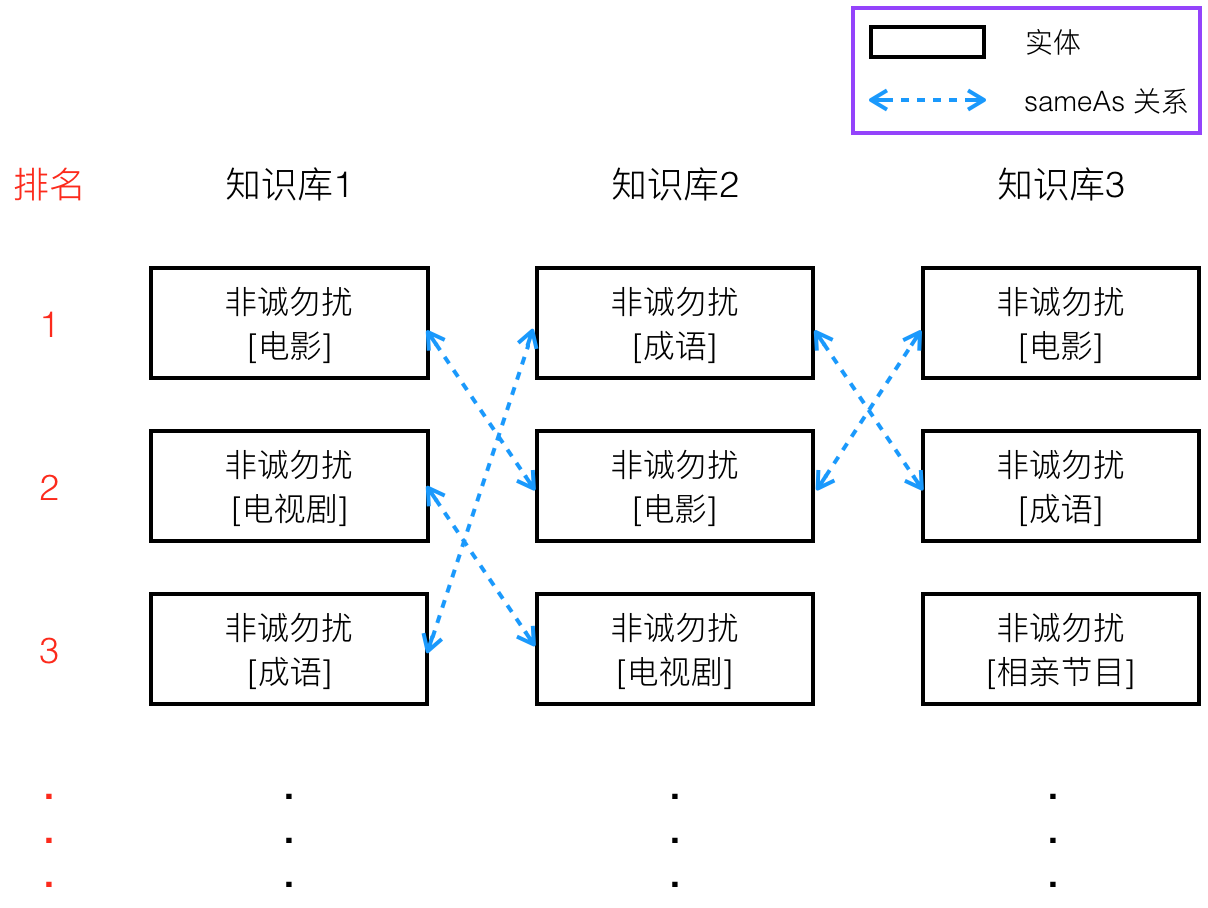
\includegraphics[width=0.8\textwidth]{img/sameas}
\caption{一个实体链接结果的实例:图~\ref{table} 中指称``非诚勿扰''在不同知识库上的候选实体的排名列表}
\label{sameas}
\end{figure}

假定有 $n$ 个不同的相互链接的知识库,两个知识库相互链接指的是二者的实体由``sameAs''关系相互关联。
对每个给定的知识库,我先使用~\ref{single} 节中提出的方法进行 Web 表格的单知识库实体链接。
对于每个指称,能够得到它的前 $n$ 个候选实体排名列表。
然后,利用不同知识库实体间的``sameAs''关系,我将候选实体排名列表中等价的实体分到一组,最后所有实体分成多个不同的组,每个组中的实体都是``sameAs''的。
例如,在图~\ref{sameas} 中,我能够得到如下的四组实体:
\begin{enumerate}[1)]
\item $Set_1=$ \{``非诚勿扰[电影]'' ($KB_1$), ``非诚勿扰[电影]'' ($KB_2$), ``非诚勿扰[电影]'' ($KB_3$)\}
\item $Set_2=$ \{``非诚勿扰[成语]'' ($KB_1$), ``非诚勿扰[成语]'' ($KB_2$), ``非诚勿扰[成语]'' ($KB_3$)\}
\item $Set_3=$ \{``非诚勿扰[电视剧]'' ($KB_1$), ``非诚勿扰[电视剧]'' ($KB_2$)\}
\item $Set_4=$ \{``非诚勿扰[相亲节目]'' ($KB_3$)\}
\end{enumerate}
有了分好组的实体的之后,计算每组实体的平均排名、最高排名和组内实体数量。
举个例子,对于 $Set_1$ 中的实体,平均排名就是 $\frac{1+2+1}{3}=1.33$,最高排名是 1,实体数量为 3。
最后,我提出了三条启发式的规则来解决多知识库实体冲突的问题,并选择一个实体分组作为给定指称的最终实体链接结果。
\begin{itemize}
  \item[$\bullet$] \textbf{规则一}: 如果一个实体分组的平均排名、最高排名在所有分组中排名最高,并且该组的实体数量不少于知识库数量的一半,那么选择这一组作为给定指称的最终实体链接结果。
  \item[$\bullet$] \textbf{规则二}: 如果有两个或多个实体分组的平均排名、最高排名相同并在所有分组中排名最高,并且这些分组的实体数量不少于知识库数量的一半,那么从这些分组中随机挑选一组作为给定指称的最终实体链接结果。
  \item[$\bullet$] \textbf{规则三}: 如果每组的实体数量都小于知识库数量的一半,那么对于给定指称,原先单知识库实体链接结果保持不变。
\end{itemize}
为了同时获得全局和局部最优的实体链接结果,我不光考虑了每个实体分组的平均排名和最高排名,还考虑每个个体 (由一个实体分组表示) 在不同知识库中的出现次数。
如果一个实体分组中的实体数量小于知识库数量的一半,这意味着这组实体表示的个体被很少的知识库所覆盖,所以平均排名并不具有说服力,也没有理由选择这个实体分组来解决多知识库的实体链接结果冲突问题。


\section{方法二: 融合}\label{approach2}
方法二尝试将方法一中的两步合并为一步,用一个统一的图模型来表示表格指称和来自多知识库的其候选实体以及实体间的``sameAs''关系。
方法二的流程与方法一无异,依旧先是指称识别,然后候选实体生成,最后实体消岐,实体消岐分为三个小步骤:构建实体消岐图,计算实体链接影响因子和迭代概率传播。
在本文中,二个方法进行指称识别和候选实体生成的方式是完全相同的,它们使用的输入数据 (表格,多知识库的各类型数据) 也是相同的。
方法二与~\ref{approach1} 节中描述的方法一的区别主要在于实体消岐图中结点定义的改变以及舍弃了~\ref{multiple} 节中提到的三条启发式规则。
在这里,我重新给出实体消岐图的定义。
\begin{itemize}
  \item[$\bullet$] \textbf{指称结点}: 这些结点指的是 Web 表格中的字符串指称
  \item[$\bullet$] \textbf{实体组结点}: 这些结点表示指称在多知识库中的基于``sameAs''的所有候选参考实体
  \item[$\bullet$] \textbf{指称-实体组边}: 一条指称-实体组边是一个指称和其候选参考实体组集合中的一个实体组之间的无向边
  \item[$\bullet$] \textbf{实体组-实体组边}: 一条实体组-实体组边是实体组之间的无向边
\end{itemize}
将方法一中提到的实体消岐图中的实体结点转变为实体组结点。
原先的实体结点只包含了一个实体,而且一张实体消岐图中所有实体结点都来自同一个知识库。
如图~\ref{edg2} 中那样,现在的实体组结点包含了一个或者多个实体,利用多知识库实体间的``sameAs''关系,将有``sameAs''关系的来自不同知识库的实体放入同一个结点,即实体组结点。
这样就将多知识库实体间的``sameAs''关系融合进实体消岐图模型了。
这种融合让我有机会实现原先方法中两步的合并。

\begin{figure}[htbp]
\centering
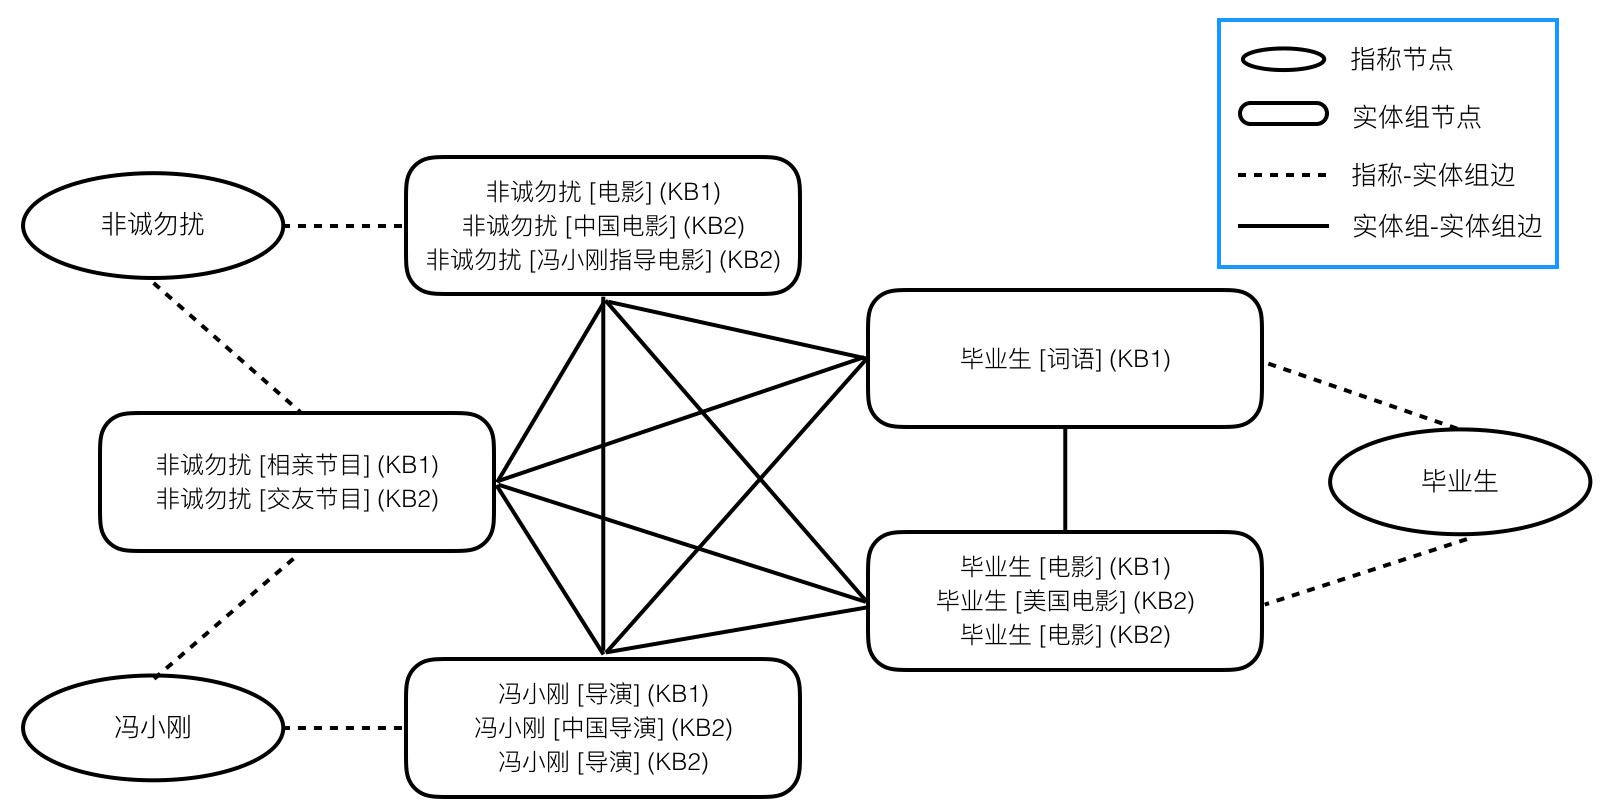
\includegraphics[width=0.9\textwidth]{img/edg2}
\caption{一个构建好的新实体消岐图示例}
\label{edg2}
\end{figure}

构建好实体消岐图之后,接着计算实体链接影响因子。
在计算一个指称 $m$ 与一个实体组 $entitySet=\{e_1 (kb1), e_2 (kb2), e_3 (kb3)\}$ 之间的\textbf{指称-实体组语义相关度}的时候,我采用的是分别计算指称 $m$ 与实体组 $entitySet$ 中每个实体的\textbf{指称-实体语义相关度},然后取平均值作为指称 $m$ 与实体组 $entitySet$ 的\textbf{指称-实体组语义相关度}。
同样的,在计算一个实体组 $entitySet1$ 与一个实体组 $entitySet2$ 之间的\textbf{实体组-实体组语义相关度}的时候,分别计算实体组 $entitySet1$ 中每个实体与实体组 $entitySet2$ 中每个实体的\textbf{实体-实体语义相关度},然后取平均值作为实体组 $entitySet1$ 与实体组 $entitySet2$ 之间的\textbf{实体组-实体组语义相关度}。
最后,在构建好的实体消岐图上,结合实体链接影响因子,使用 \ref{single} 中相同的迭代概率传播方式在实体消岐图上进行随机游走算法,得到给定指称在多知识库中的对应参考实体组作为最终的实体链接结果。


\section{sameAs 关系的学习}
在~\ref{multiple} 节中我提到导致多知识库实体链接结果冲突的一个重要原因就是``sameAs''关系的缺失。
如果不同知识库的实体间能够存在更多的``sameAs''关系,这种冲突问题可能能够被更好的解决。
为了能够学习到新的``sameAs''关系,我定义了三个特征并训练了一个监督学习分类器支持向量机\cite{tong2001support} (Support Vector Machine),其在大多数情况下\cite{fernandez2014we}有着最好的性能表现。
三个特征在下面介绍:
\begin{itemize}
  \item[$\bullet$] \textbf{同义词特征}: 这个特征用于检测两个实体字符串是否是同义词。我将两个实体字符串 $e_1$ 和 $e_2$ 输入进 BabelNet\cite{navigli2010babelnet},如果在 BabelNet 中这两个字符串有同义词关系,那么同义词特征 $isSyn = 1$,否则 $isSyn = 0$。
  \item[$\bullet$] \textbf{字符串相似度特征}: 这个特征捕捉实体间的语言学上的相关性 (Linguistic Relatedness)。两个实体 $e_1$ 和 $e_2$ 之间的字符串相似度由 $strSim(e_1, e_1)$ 表示。我使用公式~\ref{strsim} 来计算它。
  \item[$\bullet$] \textbf{实体-实体上下文相似度特征}: 对于两个来自不同知识库的实体,这个特征捕捉实体的上下文之间的相似度并且已经在公式~\ref{contsim} 中定义
\end{itemize}
除了使用支持向量机分类器来学习新的``sameAs''关系,我还考虑使用实体链接与``sameAs''进行迭代学习。
如果在最终的实体链接结果中,两个来自不同知识库的实体被同一个指称链接到,但这两个实体间并没有``sameAs''关系标记,那么此时可以为这两个实体添加``sameAs''关系。
这样就学到了新的``sameAs''关系。
而``sameAs''关系反过来又能促进实体链接,换句话说,实体链接与``sameAs''关系的学习是相互促进的。
因此让它们迭代学习既能补全多知识库间的``sameAs''关系,又能提升实体链接的质量。


\section{本章小结}
在这一章中,我首先介绍了实体链接方法中用到的两个模型:马尔科夫链模型和随机游走模型。
然后详细描述了本文提出的两个方法。
这两个方法是平行的,方法一是一个两阶段的方法,方法二是方法一的改版,其融合了方法一中的两步,这两个方法的输入和输出都是一样的。
输入都是 Web 表格和多知识库的实体数据,输出都是表格的实体链接结果,即表格中的字符串指称最终链接到的知识库中对应的参考实体。
换句话说,这两个方法中的任何一个都可以单独拿出来作为一个表格实体链接系统的核心算法。
目前实体链接的方法大体上可以分为3类:基于概率统计的方法,基于机器学习的方法和基于图模型的随机游走方法。
本文中的两个方法的核心都是属于基于图模型的随机游走方法。
这类方法的思路与另外2类方法完全不同。
它主要利用字符串指称与实体之间、实体与实体之间的语义相关性来开展实体链接的工作。

